%==============================================================================
% HIRELENS — Detailed Technical Report (Overleaf: pdfLaTeX, compile twice)
%==============================================================================
\documentclass[11pt,a4paper]{report}

\usepackage[utf8]{inputenc}
\usepackage[T1]{fontenc}
\usepackage[margin=0.9in]{geometry}
\usepackage{graphicx}
\usepackage{hyperref}
\usepackage{amsmath,amssymb}
\usepackage{booktabs}
\usepackage{enumitem}
\usepackage{xcolor}
\usepackage{listings}
\usepackage{tikz}
\usetikzlibrary{positioning,arrows.meta}
\usepackage{float}
\usepackage{caption}
\usepackage{tabularx}
\usepackage{multirow}

\hypersetup{colorlinks=true,linkcolor=blue!55!black,urlcolor=blue!55!black}

\lstset{
  basicstyle=\ttfamily\footnotesize,
  breaklines=true,
  frame=single,
  backgroundcolor=\color{gray!8},
  columns=fullflexible,
  keepspaces=true
}

\title{
  \textbf{HIRELENS}\\[0.4em]
  \large AI-Proctored Remote Interview Platform\\[0.3em]
  \large Detailed Technical Architecture, Models, and Implementation Report
}
\author{Praveen Yadav\\\url{https://github.com/eryadavpraveen/HIRELENS}}
\date{June 2026}

\begin{document}
\maketitle

\begin{abstract}
HIRELENS is a full-stack web application for integrity-monitored remote interviews. A recruiter and student conduct a peer-to-peer WebRTC video session while multiple machine-learning pipelines analyze the student's webcam and microphone in parallel. Detected anomalies become \emph{violations}: they are persisted in PostgreSQL, streamed in real time to the recruiter dashboard, and aggregated into an \emph{integrity score}. This document explains the complete system architecture, every model used, inference pipelines, API surface, security model, frontend/backend structure, and deployment topology implemented in the production codebase.
\end{abstract}

\tableofcontents
\newpage

%==============================================================================
\chapter{Introduction and Scope}
%==============================================================================

\section{Problem Statement}
Traditional video interviews (Zoom, Meet) do not provide automated proctoring: recruiters cannot systematically detect tab switching, secondary devices, identity substitution, or attention loss. HIRELENS addresses this by embedding continuous AI monitoring into the interview workflow without routing video through a central media server.

\section{Project Objectives}
\begin{enumerate}[label=\textbf{O\arabic*.}]
  \item Provide browser-based recruiter--student video calls via WebRTC.
  \item Run parallel CV/speech checks: face presence, objects, identity, head/eye attention, voice.
  \item Record violations with timestamps and expose live recruiter dashboards.
  \item Compute a transparent integrity score from violation categories.
  \item Enforce role-based access (recruiter vs student) with JWT authentication.
  \item Separate heavy ML inference into dedicated services for maintainability.
\end{enumerate}

\section{System Boundaries}
\begin{itemize}
  \item \textbf{In scope:} Interview lifecycle, monitoring, WebRTC signaling relay, reports, verification (photo + voice).
  \item \textbf{Out of scope / partial:} Lip-sync anti-spoofing (mouth-open ratio only), TURN servers (STUN only), automated email in all environments.
\end{itemize}

%==============================================================================
\chapter{High-Level Architecture}
%==============================================================================

\section{Runtime Components}

\begin{table}[H]
\centering
\caption{Production runtime tiers}
\small
\begin{tabularx}{\textwidth}{@{}lXcl@{}}
\toprule
\textbf{Component} & \textbf{Responsibility} & \textbf{Port} & \textbf{Hosting} \\
\midrule
Frontend SPA & UI, monitoring loops, WebRTC client & 5173 / HTTPS & Vercel \\
Backend API & REST, WebSocket signaling, CV/identity/YOLO & 8000 & VPS / Oracle VM \\
Attention service & MediaPipe landmarks, Resemblyzer voice & 8001 & VPS / Oracle VM \\
PostgreSQL & Users, interviews, violations, voiceprints & 5432 & Supabase \\
\bottomrule
\end{tabularx}
\end{table}

\section{Traffic Separation}
\begin{itemize}
  \item \textbf{Media plane:} WebRTC peer-to-peer (UDP/TCP negotiated by ICE). Never stored on server.
  \item \textbf{Control plane:} WebSocket JSON (SDP, ICE, monitoring events).
  \item \textbf{Inference plane:} HTTP multipart JPEG/WebM uploads from student browser to backend and attention service.
  \item \textbf{Persistence plane:} SQL writes for violations, participants, voiceprints.
\end{itemize}

\section{Architecture Diagram}

\begin{figure}[H]
\centering
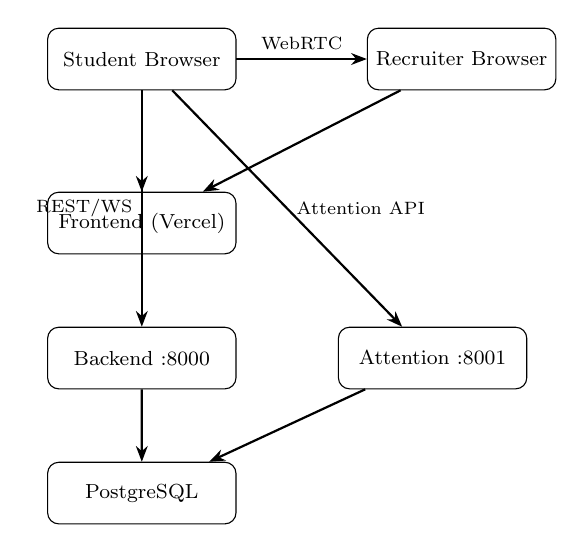
\begin{tikzpicture}[
  scale=0.92, transform shape,
  box/.style={draw, rounded corners, align=center, minimum width=2.6cm, minimum height=0.85cm, font=\footnotesize},
  arr/.style={-{Stealth[length=2mm]}, thick}
]
  \node[box] (stu) {Student Browser};
  \node[box, right=1.8cm of stu] (rec) {Recruiter Browser};
  \node[box, below=1.4cm of stu] (vercel) {Frontend (Vercel)};
  \node[box, below=of vercel] (api) {Backend :8000};
  \node[box, right=1.4cm of api] (att) {Attention :8001};
  \node[box, below=of api] (db) {PostgreSQL};
  \draw[arr] (stu) -- node[above,font=\scriptsize]{WebRTC} (rec);
  \draw[arr] (stu) -- (vercel);
  \draw[arr] (rec) -- (vercel);
  \draw[arr] (stu) -- node[left,font=\scriptsize]{REST/WS} (api);
  \draw[arr] (stu) -- node[right,font=\scriptsize]{Attention API} (att);
  \draw[arr] (api) -- (db);
  \draw[arr] (att) -- (db);
\end{tikzpicture}
\caption{Logical deployment. Only signaling and API traffic hit the backend; video is peer-to-peer.}
\end{figure}

%==============================================================================
\chapter{Repository Structure}
%==============================================================================

\begin{verbatim}
HIRELENS/
  frontend/src/
    pages/Student/     JoinInterview, VerificationPage, StudentInterviewRoom
    pages/Recruiter/   CreateInterview, RecruiterInterviewRoom, ...
    hooks/             useWebRTC.js, useMonitoring.js
    services/          api.js, interviewService.js, monitoringService.js
    utils/violations.js   Integrity engine (client-side)
  backend/app/
    api/               interview, participant, violation, signaling, auth, ...
    services/          face_detector, object_detector, face_verification, ...
    models/            SQLAlchemy ORM models
    migrations/        SQL migration files
  attention_service/
    services/          face_landmarker_service, voice_verifier, ...
    models/            face_landmarker.task (TFLite asset)
  deploy/              oracle-vm-setup.sh, nginx, systemd units
  docs/                Documentation and this report
\end{verbatim}

%==============================================================================
\chapter{Technology Stack}
%==============================================================================

\begin{table}[H]
\centering
\caption{Major dependencies (representative versions from requirements)}
\small
\begin{tabularx}{\textwidth}{@{}lX@{}}
\toprule
\textbf{Layer} & \textbf{Libraries / tools} \\
\midrule
Frontend & React 19, Vite, Redux Toolkit, Axios, React Router, Tailwind, Framer Motion, jsPDF \\
Backend API & FastAPI 0.137, Uvicorn/Gunicorn, SQLAlchemy 2.x, python-jose, bcrypt, psycopg2 \\
Backend ML & OpenCV, MediaPipe 0.10+, DeepFace (FaceNet), Ultralytics YOLOv8, TensorFlow 2.x \\
Attention ML & MediaPipe Tasks Face Landmarker (TFLite), Resemblyzer, PyTorch 2.x, NumPy \\
Infrastructure & Nginx reverse proxy, systemd services, Supabase PostgreSQL \\
\bottomrule
\end{tabularx}
\end{table}

%==============================================================================
\chapter{Authentication and Authorization}
%==============================================================================

\section{Token Model}
\begin{itemize}
  \item \textbf{Access token} (JWT): default 15 minutes. Payload: \texttt{sub} (user UUID), \texttt{role}, \texttt{type=access}.
  \item \textbf{Refresh token}: stored hashed in \texttt{refresh\_tokens}; rotated on \texttt{POST /auth/refresh}.
  \item Browser storage: \texttt{hirelens\_token}, \texttt{hirelens\_refresh\_token}, \texttt{hirelens\_user}.
\end{itemize}

\section{Login Flow}
\begin{enumerate}
  \item Client \texttt{POST /auth/login} with email/password.
  \item Server verifies bcrypt hash, issues access + refresh tokens.
  \item \texttt{api.js} interceptor attaches \texttt{Authorization: Bearer} header.
  \item On 401, client attempts refresh; on failure redirects to login.
\end{enumerate}

\section{WebSocket Authorization}
Connection URL: \texttt{/ws/interview/\{id\}?role=student|recruiter\&token=\{JWT\}}.

Server validates:
\begin{itemize}
  \item Token signature and \texttt{type=access}.
  \item User role matches query \texttt{role}.
  \item Recruiter: \texttt{interview.recruiter\_id == user.id}.
  \item Student: row exists in \texttt{participants} for this interview.
\end{itemize}

\section{Interview Authorization Matrix}

\begin{table}[H]
\centering
\small
\begin{tabularx}{\textwidth}{@{}lXX@{}}
\toprule
\textbf{Endpoint} & \textbf{Recruiter} & \textbf{Student} \\
\midrule
Create interview & Owner account & Denied \\
\texttt{GET /interviews/\{id\}} & If owner & If participant \\
\texttt{GET /join-preview} & Denied & If interview exists \& not completed \\
\texttt{POST /join} & Denied & Creates participant row \\
Record violation & Denied & If participant \\
WebSocket room & If owner & If participant \\
\bottomrule
\end{tabularx}
\end{table}

%==============================================================================
\chapter{Database Design}
%==============================================================================

\section{Entity Relationships}
\begin{itemize}
  \item \texttt{users} (1) $\rightarrow$ (N) \texttt{interviews} as recruiter.
  \item \texttt{interviews} (1) $\rightarrow$ (N) \texttt{participants}, \texttt{violations}.
  \item \texttt{participants} links \texttt{student\_id} to \texttt{interview\_id}.
  \item \texttt{voiceprints} keyed by \texttt{candidate\_id} (interview UUID string).
\end{itemize}

\section{Table Definitions}

\begin{table}[H]
\centering
\small
\caption{Core tables}
\begin{tabularx}{\textwidth}{@{}lX@{}}
\toprule
\textbf{Table} & \textbf{Key columns} \\
\midrule
\texttt{users} & id, name, email, password\_hash, role \\
\texttt{interviews} & id, title, recruiter\_id, status, completed\_at, start/end\_time \\
\texttt{participants} & id, interview\_id, student\_id, joined\_at \\
\texttt{violations} & id, interview\_id, student\_id, type, duration, confidence, timestamp \\
\texttt{voiceprints} & candidate\_id (PK), embedding (JSONB), timestamps \\
\texttt{refresh\_tokens} & id, user\_id, token\_hash, expires\_at, revoked \\
\bottomrule
\end{tabularx}
\end{table}

Migrations applied automatically at backend startup from \texttt{backend/migrations/}.

%==============================================================================
\chapter{Backend API Reference}
%==============================================================================

\section{Authentication Endpoints}
\begin{tabularx}{\textwidth}{@{}lX@{}}
\toprule
\texttt{POST /auth/register} & Register student or recruiter \\
\texttt{POST /auth/login} & Returns access + refresh tokens \\
\texttt{POST /auth/refresh} & Rotate refresh token \\
\texttt{POST /auth/logout} & Revoke refresh token \\
\texttt{GET /auth/me} & Current user profile \\
\texttt{POST /auth/forgot-password} & Issue reset token \\
\texttt{POST /auth/reset-password} & Consume reset token \\
\bottomrule
\end{tabularx}

\section{Interview Endpoints}
\begin{tabularx}{\textwidth}{@{}lX@{}}
\toprule
\texttt{POST /interviews/} & Create (recruiter) \\
\texttt{GET /interviews/} & List (scoped by role) \\
\texttt{GET /interviews/\{id\}} & Detail (authorized) \\
\texttt{GET /interviews/\{id\}/join-preview} & Pre-join safe fields (student) \\
\texttt{POST /interviews/\{id\}/join} & Insert participant (student) \\
\texttt{PATCH /interviews/\{id\}/complete} & Lock interview; broadcast WS \\
\texttt{DELETE /interviews/\{id\}} & Cascade delete + cleanup \\
\texttt{GET /interviews/\{id\}/participants} & List participants \\
\bottomrule
\end{tabularx}

\section{Computer Vision Endpoints}
\begin{tabularx}{\textwidth}{@{}lX@{}}
\toprule
\texttt{POST /cv/check-face} & Haar cascade face count \\
\texttt{POST /identity/verify-identity} & DeepFace FaceNet match \\
\texttt{POST /object-detection/check} & YOLOv8n object detection \\
\texttt{POST /verification/upload} & Store reference photo \\
\bottomrule
\end{tabularx}

\section{Violations and Reports}
\begin{tabularx}{\textwidth}{@{}lX@{}}
\toprule
\texttt{POST /violations/} & Persist violation (student participant) \\
\texttt{GET /violations/\{interview\_id\}} & List violations \\
\texttt{GET /reports/} & Recruiter report list \\
\texttt{GET /reports/\{id\}} & Report with event timeline \\
\texttt{POST /reports/generate/\{id\}} & Generate report snapshot \\
\bottomrule
\end{tabularx}

%==============================================================================
\chapter{Attention Service API}
%==============================================================================

\begin{tabularx}{\textwidth}{@{}lX@{}}
\toprule
\texttt{POST /attention/analyze} & Full landmark + attention pipeline on JPEG \\
\texttt{POST /voice/register} & JWT student; store embedding in DB \\
\texttt{POST /voice/verify} & Compare live audio to stored embedding \\
\texttt{DELETE /voice/\{candidate\_id\}} & Remove voiceprint (interview delete) \\
\bottomrule
\end{tabularx}

\textbf{Startup:} Lazy model loading; \texttt{lifespan} warms Face Landmarker and VoiceEncoder; failures log Python tracebacks.

%==============================================================================
\chapter{WebRTC and Signaling Protocol}
%==============================================================================

\section{Peer Connection Establishment}
\begin{enumerate}
  \item Both peers connect WebSocket with JWT.
  \item Server sends \texttt{room-joined} with participant list.
  \item When student present, recruiter calls \texttt{createOffer()}.
  \item \texttt{offer} $\rightarrow$ student \texttt{answer} $\rightarrow$ ICE candidates exchanged.
  \item \texttt{ontrack} receives remote MediaStream for video elements.
\end{enumerate}

\section{Relayed WebSocket Message Types}

\begin{table}[H]
\centering
\small
\begin{tabularx}{\textwidth}{@{}lX@{}}
\toprule
\textbf{Type} & \textbf{Purpose} \\
\midrule
\texttt{offer}, \texttt{answer}, \texttt{ice-candidate} & WebRTC signaling \\
\texttt{monitoring-event} & Violation event JSON to recruiter \\
\texttt{status-update} & Live monitoring badge updates \\
\texttt{room-joined}, \texttt{peer-joined}, \texttt{peer-left} & Presence \\
\texttt{interview-completed} & Session teardown message \\
\bottomrule
\end{tabularx}
\end{table}

\section{ICE Configuration}
Google STUN: \texttt{stun:stun.l.google.com:19302}. Production may require TURN for restrictive NAT.

\section{Local Media Controls}
\texttt{MediaStreamTrack.enabled = false} mutes camera/mic without closing PeerConnection.

%==============================================================================
\chapter{Machine Learning Models --- Detailed Specification}
%==============================================================================

This chapter documents each model: mathematical basis, implementation file, inference steps, thresholds, and violation mapping.

%------------------------------------------------------------------------------
\section{OpenCV Haar Cascade Face Detector}
%------------------------------------------------------------------------------

\subsection{Theoretical Background}
Viola--Jones (2001) uses AdaBoost-trained Haar-like features with a cascade of weak classifiers for fast frontal-face detection. It is classical computer vision (not deep learning): integral images enable real-time scanning at multiple scales.

\subsection{Implementation}
\texttt{backend/app/services/face\_detector.py}, cascade file \texttt{haarcascade\_frontalface\_default.xml}.

\subsection{Algorithm}
\begin{enumerate}
  \item Decode uploaded JPEG to BGR matrix.
  \item Grayscale conversion.
  \item \texttt{detectMultiScale(gray, scaleFactor=1.1, minNeighbors=5, minSize=(30,30))}.
  \item Return bounding box count.
\end{enumerate}

\subsection{API Mapping}
\texttt{POST /cv/check-face} returns \texttt{status}: \texttt{NO\_FACE} (0), \texttt{FACE\_PRESENT} (1), \texttt{MULTIPLE\_FACE} ($\geq 2$). Frontend reports \texttt{MULTIPLE\_PERSON\_FACE} every 2\,s when applicable.

\subsection{Limitations}
Sensitive to pose/lighting; may miss profile faces; can false-positive on patterns. Complemented by YOLO person count.

%------------------------------------------------------------------------------
\section{Ultralytics YOLOv8n}
%------------------------------------------------------------------------------

\subsection{Theoretical Background}
YOLO (You Only Look Once) performs single-pass object detection: the network divides the image into a grid and predicts bounding boxes and class probabilities simultaneously. YOLOv8-nano is the smallest variant, optimized for edge/CPU deployment.

\subsection{Model Asset}
\texttt{backend/yolov8n.pt} --- COCO-pretrained weights (80 classes).

\subsection{Implementation}
\texttt{object\_detector.py}: \texttt{model = YOLO("yolov8n.pt")} at import; \texttt{model(image\_path)} per request.

\subsection{Detected Classes (HIRELENS mapping)}
\begin{table}[H]
\centering
\small
\begin{tabular}{@{}lll@{}}
\toprule
COCO class & Field & Violation \\
\midrule
cell phone & phone=true & OBJECT\_PHONE \\
book & book\_count++ & OBJECT\_BOOK \\
laptop & laptop\_count++ & OBJECT\_DEVICE \\
person & person\_count & MULTIPLE\_PERSON\_YOLO if $\geq 2$ \\
\bottomrule
\end{tabular}
\end{table}

\subsection{Inference Frequency}
Frontend object loop: every 3\,s. JPEG quality 0.7 from canvas capture.

%------------------------------------------------------------------------------
\section{DeepFace FaceNet Identity Verification}
%------------------------------------------------------------------------------

\subsection{Theoretical Background}
FaceNet (Schroff et al., 2015) learns a mapping $f(x) \in \mathbb{R}^{128}$ such that Euclidean distance between embeddings of the same person is small and large for different persons. DeepFace wraps FaceNet with OpenCV face detection for alignment.

\subsection{Configuration}
\begin{itemize}
  \item \texttt{model\_name="Facenet"}
  \item \texttt{detector\_backend="opencv"}
  \item \texttt{enforce\_detection=False}
\end{itemize}

\subsection{Pipeline}
\begin{enumerate}
  \item Reference: \texttt{uploads/verification/\{candidate\_id\}.jpg} from verification page.
  \item Live frame saved to temp JPEG.
  \item \texttt{DeepFace.verify(reference, current)} $\rightarrow$ distance vs threshold $\rightarrow$ \texttt{verified} boolean.
\end{enumerate}

\subsection{Violation}
\texttt{IDENTITY\_MISMATCH} when \texttt{verified == false}. Loop interval: 4\,s.

%------------------------------------------------------------------------------
\section{MediaPipe Face Landmarker (Attention Service)}
%------------------------------------------------------------------------------

\subsection{Theoretical Background}
MediaPipe Face Landmarker is a TensorFlow Lite pipeline predicting 478 3D facial landmarks, blendshape coefficients, and a facial transformation matrix (head pose in camera space). Inference uses XNNPACK CPU delegate.

\subsection{Model File}
\texttt{attention\_service/models/face\_landmarker.task} ($\sim$3.7\,MB).

\subsection{Initialization Options}
\begin{itemize}
  \item \texttt{output\_face\_blendshapes=True}
  \item \texttt{output\_facial\_transformation\_matrixes=True}
  \item \texttt{num\_faces=1}
  \item Lazy load via \texttt{get\_landmarker()}; warmed in FastAPI lifespan.
\end{itemize}

\subsection{Sub-pipeline A: Head Pose}
\texttt{head\_tracker.py} reads $4 \times 4$ transformation matrix:
\begin{itemize}
  \item yaw from matrix element; LEFT if yaw $< -0.20$, RIGHT if $> 0.20$.
  \item pitch: UP if $< -0.10$, DOWN if $> 0.25$.
\end{itemize}

\subsection{Sub-pipeline B: Eye Gaze}
\texttt{eye\_tracker.py} uses landmarks 33, 133 (eye corners), 468 (iris):
\[
\text{ratio} = \frac{x_{\text{iris}} - x_{\text{left}}}{x_{\text{right}} - x_{\text{left}}}
\]
LEFT if ratio $< 0.35$; RIGHT if $> 0.55$; else CENTER.

\subsection{Sub-pipeline C: Eye Closure (EAR)}
Eye Aspect Ratio:
\[
\text{EAR} = \frac{\text{vertical eye distance}}{\text{horizontal eye distance}}
\]
Eyes closed if EAR $< 0.18$ (landmarks 159, 145, 33, 133).

\subsection{Sub-pipeline D: Mouth Opening}
\texttt{lipsync\_detector.py}: mouth gap / face width; \texttt{mouth\_open} if ratio $> 0.04$. \textbf{Not} lip-sync verification.

\subsection{Sub-pipeline E: Attention Fusion}
\texttt{attention\_engine.py} rule-based:
\begin{itemize}
  \item Non-center horizontal/vertical head $\rightarrow$ \texttt{HEAD\_LEFT/RIGHT/UP/DOWN}.
  \item Non-center eye direction $\rightarrow$ \texttt{EYE\_LEFT/RIGHT}.
  \item Eyes closed $\rightarrow$ \texttt{EYES\_CLOSED}, \texttt{drowsiness\_alert}.
\end{itemize}

\subsection{API Response}
\texttt{POST /attention/analyze} returns landmark count, yaw/pitch, eye direction, EAR, attention flags, mouth ratio. Frontend attention loop: 1\,s.

%------------------------------------------------------------------------------
\section{MediaPipe Face Mesh (Backend Auxiliary)}
%------------------------------------------------------------------------------

\texttt{backend/app/services/head\_pose.py} uses legacy Face Mesh (468 landmarks). Nose $x$-coordinate thresholds: $<0.40$ LEFT, $>0.60$ RIGHT. Used in tests/auxiliary paths; primary attention path uses Face Landmarker service.

%------------------------------------------------------------------------------
\section{Resemblyzer VoiceEncoder}
%------------------------------------------------------------------------------

\subsection{Theoretical Background}
Resemblyzer implements a GE2E (Generalized End-to-End) speaker embedding network. The encoder maps variable-length utterances to a fixed-dimensional unit vector suitable for cosine/dot-product similarity.

\subsection{Implementation}
\texttt{voice\_verifier.py}: PyTorch \texttt{VoiceEncoder()}, lazy singleton.

\subsection{Registration}
\begin{enumerate}
  \item \texttt{preprocess\_wav(path)}: resample, normalize volume, trim silence.
  \item \texttt{embed\_utterance(wav)} $\rightarrow$ vector $\mathbf{e}$.
  \item Store in \texttt{voiceprints.embedding} (JSONB) keyed by interview/candidate id.
\end{enumerate}

\subsection{Verification}
$\text{similarity} = \mathbf{e}_{\text{stored}} \cdot \mathbf{e}_{\text{live}}$ (dot product on normalized embeddings).

\subsection{Thresholds}
\begin{table}[H]
\centering
\begin{tabular}{@{}ll@{}}
\toprule
Similarity & Status \\
\midrule
$\geq 0.85$ & VERIFIED \\
$[0.75, 0.85)$ & SUSPICIOUS (no violation) \\
$< 0.75$ & VOICE\_MISMATCH \\
\bottomrule
\end{tabular}
\end{table}

\subsection{Monitoring}
5\,s audio capture (\texttt{VOICE\_RECORD\_MS}), verify every 1\,s cooldown after cycle completes.

%------------------------------------------------------------------------------
\section{Models Summary}
%------------------------------------------------------------------------------

\begin{table}[H]
\centering
\small
\caption{Consolidated model inventory}
\begin{tabularx}{\textwidth}{@{}llll@{}}
\toprule
\textbf{Model} & \textbf{Type} & \textbf{Service} & \textbf{Output} \\
\midrule
Haar Cascade & Classical CV & Backend & Face count \\
YOLOv8n & CNN detector & Backend & COCO classes \\
FaceNet & Deep embedding & Backend & Identity match \\
Face Landmarker & TFLite landmarks & Attention & Pose, gaze, EAR \\
Face Mesh & MediaPipe & Backend aux & Head direction \\
VoiceEncoder & PyTorch GE2E & Attention & Speaker embedding \\
\bottomrule
\end{tabularx}
\end{table}

%==============================================================================
\chapter{Monitoring Pipeline (Student Browser)}
%==============================================================================

\section{Loop Scheduling}
Five independent async loops in \texttt{useMonitoring.js}; each awaits completion before sleeping.

\begin{table}[H]
\centering
\caption{Monitoring loop parameters}
\begin{tabular}{@{}llll@{}}
\toprule
\textbf{Loop} & \textbf{Interval} & \textbf{Endpoint} & \textbf{Auth} \\
\midrule
Attention & 1\,s & Attention /attention/analyze & JWT on attention client \\
Face & 2\,s & Backend /cv/check-face & JWT \\
Object & 3\,s & Backend /object-detection/check & JWT \\
Identity & 4\,s & Backend /identity/verify-identity & JWT \\
Voice & 1\,s cooldown & Attention /voice/verify & JWT \\
\bottomrule
\end{tabular}
\end{table}

\section{Event Emission (\texttt{report()})}
For each violation type:
\begin{enumerate}
  \item Dedup: skip if same type within 5\,s (\texttt{EVENT\_DEDUPE\_MS}).
  \item WebSocket \texttt{\{type: "monitoring-event", event: \{type, timestamp, ...\}\}}.
  \item \texttt{POST /violations/} with interview\_id, type, duration, confidence.
  \item Student UI: \textbf{no toast} (silent recording). Fullscreen uses dedicated overlay only.
\end{enumerate}

\section{Environment Proctoring (Browser Events)}
\begin{table}[H]
\centering
\small
\begin{tabularx}{\textwidth}{@{}lXl@{}}
\toprule
\textbf{Event} & \textbf{Behavior} & \textbf{Violation} \\
\midrule
\texttt{visibilitychange} hidden & Complete interview, end session & TAB\_SWITCH \\
\texttt{blur} & Record only & WINDOW\_BLUR \\
\texttt{resize} & Record only & WINDOW\_RESIZE \\
\texttt{fullscreenchange} exit & Blocking overlay + record & FULLSCREEN\_EXIT \\
\bottomrule
\end{tabularx}
\end{table}

%==============================================================================
\chapter{Violations and Integrity Engine}
%==============================================================================

\section{Raw Event Types (Examples)}
\texttt{HEAD\_LEFT}, \texttt{EYE\_RIGHT}, \texttt{NO\_FACE}, \texttt{OBJECT\_PHONE}, \texttt{MULTIPLE\_PERSON\_FACE}, \texttt{MULTIPLE\_PERSON\_YOLO}, \texttt{VOICE\_MISMATCH}, \texttt{IDENTITY\_MISMATCH}, \texttt{WINDOW\_BLUR}, \texttt{FULLSCREEN\_EXIT}, \texttt{TAB\_SWITCH}, etc.

\section{Category Mapping}
\texttt{frontend/src/utils/violations.js} maps raw types to 11 categories via \texttt{categorizeViolation()}.

\section{Category Weights and Severity}

\begin{table}[H]
\centering
\small
\caption{Integrity penalty weights per category}
\begin{tabular}{@{}llrl@{}}
\toprule
\textbf{Category} & \textbf{Severity} & \textbf{Weight} & \textbf{Example raw types} \\
\midrule
head & Yellow & 1 & HEAD\_LEFT, HEAD\_RIGHT \\
eye & Yellow & 1 & EYE\_LEFT, EYES\_CLOSED \\
no\_face & Orange & 3 & NO\_FACE \\
window & Orange & 2 & WINDOW\_BLUR, WINDOW\_RESIZE \\
fullscreen & Orange & 3 & FULLSCREEN\_EXIT \\
object & Red & 5 & OBJECT\_PHONE, OBJECT\_BOOK \\
multiple\_person & Purple & 6 & max(FACE, YOLO counts) \\
voice & Red & 5 & VOICE\_MISMATCH \\
lipsync & Red & 4 & LIP\_SYNC\_* (if emitted) \\
identity & Purple & 8 & IDENTITY\_MISMATCH \\
tab\_switch & Purple & 4 & TAB\_SWITCH \\
\bottomrule
\end{tabular}
\end{table}

\section{Integrity Score Formula}
Let $c_i$ be deduplicated count for category $i$, $w_i$ its weight:
\[
\text{penalty} = \sum_i w_i \cdot c_i,\quad
\text{score} = \max(0, \min(100, \mathrm{round}(100 - \text{penalty})))
\]

\section{Evaluation Bands}
\begin{tabular}{@{}ll@{}}
85--100 & EXCELLENT \\
70--84 & GOOD \\
50--69 & SUSPICIOUS \\
0--49 & HIGH RISK \\
\end{tabular}

\section{Multiple Person De-duplication}
\texttt{MULTIPLE\_PERSON\_FACE} and \texttt{MULTIPLE\_PERSON\_YOLO} counted separately in timeline; summary uses $\max(\text{face}, \text{yolo})$ to avoid double penalty for one physical event.

%==============================================================================
\chapter{Frontend Application Detail}
%==============================================================================

\section{Route Map}
\begin{itemize}
  \item Public: \texttt{/}, \texttt{/login}, \texttt{/register}
  \item Student: \texttt{/student/join}, \texttt{/student/interview/:id/verify}, \texttt{/student/interview/:id}
  \item Recruiter: \texttt{/recruiter/create}, \texttt{/recruiter/interview/:id}, \texttt{/recruiter/reports/:id}
\end{itemize}

\section{Redux Slices}
\texttt{authSlice}, \texttt{interviewSlice}, \texttt{monitoringSlice} (liveEvents, statuses, warnings), \texttt{reportSlice}.

\section{Recruiter Interview Room Components}
\texttt{VideoStream} (candidate + self), \texttt{ViolationTimeline}, \texttt{ViolationDashboard}, \texttt{IntegrityDashboard}, \texttt{MonitoringPanel}, \texttt{RecruiterInterviewControls} (camera/mic/end/report).

\section{Student Interview Room}
Pre-start lobby $\rightarrow$ fullscreen start $\rightarrow$ monitoring active. \texttt{FullscreenExitOverlay} blocks UI until fullscreen restored.

%==============================================================================
\chapter{End-to-End User Flows}
%==============================================================================

\section{Recruiter Flow (Step-by-Step)}
\begin{enumerate}
  \item Register/login as recruiter.
  \item Create interview (\texttt{POST /interviews/}) with title, schedule.
  \item Share interview UUID with student.
  \item Open \texttt{/recruiter/interview/\{id\}}.
  \item WebSocket connects; wait for student peer.
  \item Observe live violations, integrity score, monitoring badges.
  \item Optional: generate report; end session or mark complete.
\end{enumerate}

\section{Student Flow (Step-by-Step)}
\begin{enumerate}
  \item Register/login as student.
  \item Join page: enter interview ID $\rightarrow$ \texttt{join-preview} validates $\rightarrow$ \texttt{POST join}.
  \item Verification: upload reference photo + register voice (attention service).
  \item Interview room: start $\rightarrow$ fullscreen $\rightarrow$ WebRTC + monitoring loops.
  \item Tab switch terminates interview; fullscreen exit shows recovery dialog.
  \item Violations recorded silently; recruiter sees all alerts.
\end{enumerate}

%==============================================================================
\chapter{Deployment Architecture}
%==============================================================================

\section{Recommended Production Topology}
\begin{itemize}
  \item Frontend: Vercel, root \texttt{frontend/}, env \texttt{VITE\_*}.
  \item Database: Supabase PostgreSQL.
  \item Backend + Attention: Ubuntu VPS (4--8\,GB RAM minimum), Nginx reverse proxy, systemd services from \texttt{deploy/}.
\end{itemize}

\section{Environment Variables}

\begin{table}[H]
\centering
\small
\begin{tabularx}{\textwidth}{@{}lX@{}}
\toprule
\textbf{Variable} & \textbf{Purpose} \\
\midrule
\texttt{DATABASE\_URL} & PostgreSQL connection \\
\texttt{SECRET\_KEY}, \texttt{ALGORITHM} & JWT signing \\
\texttt{FRONTEND\_URL} & CORS + password reset links \\
\texttt{VITE\_API\_BASE\_URL} & Frontend REST base \\
\texttt{VITE\_ATTENTION\_SERVICE\_URL} & Attention API base \\
\texttt{VITE\_WS\_BASE\_URL} & WebSocket base (wss in prod) \\
\texttt{VITE\_USE\_MOCK} & Must be \texttt{false} in production \\
\bottomrule
\end{tabularx}
\end{table}

\section{HTTPS Requirement}
Browsers require secure context for \texttt{getUserMedia}, fullscreen API, and reliable WebRTC in production.

%==============================================================================
\chapter{Conclusion and Future Work}
%==============================================================================

HIRELENS combines classical CV, object detection, deep face verification, dense facial landmarks, and speaker embeddings in a unified browser-orchestrated monitoring pipeline with peer-to-peer video and centralized audit storage.

\subsection{Known Limitations}
\begin{itemize}
  \item No true lip-sync anti-spoofing model.
  \item STUN-only WebRTC may fail on some networks (TURN needed).
  \item Server RAM requirements high for concurrent ML inference.
  \item Haar + YOLO may produce correlated multiple-person signals (mitigated by de-duplication).
\end{itemize}

\subsection{Future Enhancements}
TURN integration, GPU inference, ONNX export for faster cold starts, centralized model registry, lip-sync deep model, recruiter analytics export.

%==============================================================================
\appendix
\chapter{Compilation Instructions}
%==============================================================================

Upload to Overleaf; compiler: \textbf{pdfLaTeX}. Click Recompile \textbf{twice} for table of contents.

\begin{verbatim}
pdflatex HIRELENS_TECHNICAL_REPORT.tex
pdflatex HIRELENS_TECHNICAL_REPORT.tex
\end{verbatim}

\chapter{Key Source File Index}
\begin{itemize}
  \item \texttt{frontend/src/hooks/useMonitoring.js} --- monitoring loops
  \item \texttt{frontend/src/hooks/useWebRTC.js} --- WebRTC + signaling
  \item \texttt{frontend/src/utils/violations.js} --- integrity engine
  \item \texttt{backend/app/api/signaling.py} --- WebSocket relay
  \item \texttt{backend/app/services/object\_detector.py} --- YOLO
  \item \texttt{backend/app/services/face\_verification.py} --- DeepFace
  \item \texttt{attention\_service/services/face\_landmarker\_service.py}
  \item \texttt{attention\_service/services/voice\_verifier.py}
  \item \texttt{docs/HIRELENS\_DOCUMENTATION.md} --- Markdown companion doc
\end{itemize}

\end{document}
